\DiaryEntry{Continuity, 1}{2016-01-24}{Topology}

\subsubsection{Classical Definition}

Given any subset \(\mathcal{S}\) of \(\mathcal{R}\), a function
\(f : \mathcal{S} \rightarrow \mathcal{R}\) is continuous at a point
\(a\) in its domain \(\mathcal{S}\) if: For every \(\epsilon > 0\), it
is possible to find a \(\delta > 0\) such that

\[
| f(x) - f(a) | < \epsilon \,\, \text{for} \,\, |x-a| < \delta
\]

The idea is as follows: We allow for a certain variation \(\epsilon\) of
the function values and ask for the interval in which this variation
takes place. For a fixed variation, we are allowed to choose an
arbitrary small \(\delta\); however, it is important, that such a
\(\delta\) exists and can be found at all.

The Figure below shows a function being continuous at \(x=a\) on the
left, and a function being discontinuous at \(x=a\).

On the left, we can \textbf{always} find a \(\delta\) for every value
\(\epsilon\) we choose. On the right, it is not possible to find a
\(\delta\) for values of \(\epsilon\) smaller than the jump at \(x=a\).

\begin{figure}[H]
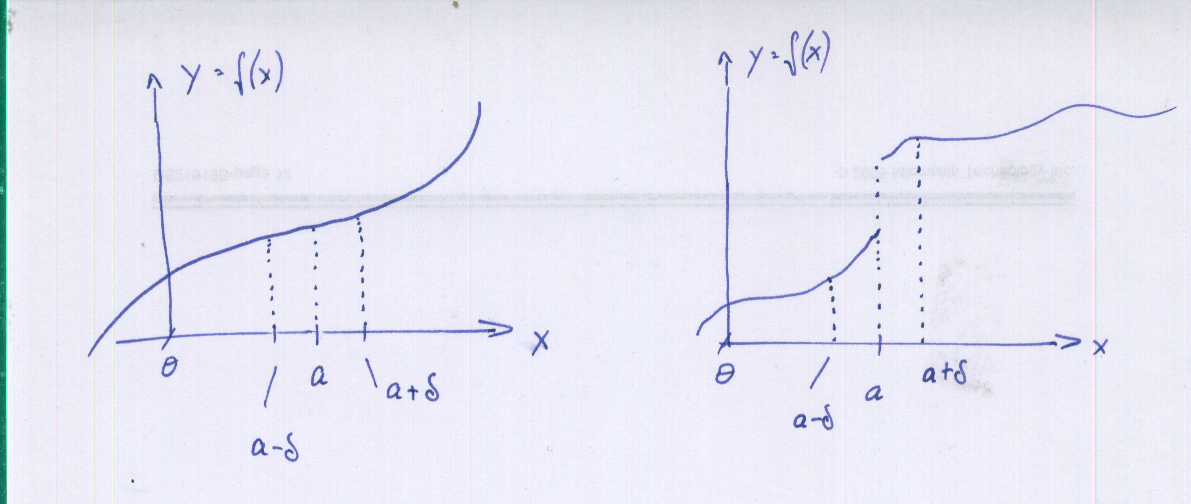
\includegraphics[scale=0.7]{images/continuity_01.png}
\end{figure}

\subsubsection{Example}

Consider the function \(f(x)=x^2\). At \(x=2\), we have the following
two equations:


\begin{align}
(2+\epsilon)^2 & = 2+\delta \\
(2-\epsilon)^2 & = 2-\delta
\end{align}


For \textbf{any value} \(\epsilon\), we can solve both equations for
\(\delta\) (the ``final'' \(\delta\) is the larger of the two).

Now consider the function given by

\[
f(x) = \begin{cases}
0 & \mbox{if } x \leq 0 \\
1 & \mbox{if } x > 0 \end{cases}
\]

If we consider \(x=0\), where \(y=0\), then we can choose a value of
\(\epsilon=1/2\) for which no value \(\delta\) can be found.
